\documentclass[sigconf]{acmart}

\usepackage{booktabs} % For formal tables


\begin{document}
\title{Visualizing User Behavior on the Places and Spaces Website}

\author{Avadhoot Agasti}
\affiliation{School of Informatics and Computing, Bloomington, IN 47408, U.S.A.}
\email{aagasti@indiana.edu}

\author{Sharad Ghule}
\affiliation{School of Informatics and Computing, Bloomington, IN 47408, U.S.A.}
\email{sghule@indiana.edu}

\author{Shreyas Rawagad}
\affiliation{School of Informatics and Computing, Bloomington, IN 47408, U.S.A.}
\email{srawagad@indiana.edu}

\author{Leonard Mwangi}
\affiliation{School of Informatics and Computing, Bloomington, IN 47408, U.S.A.}
\email{lmwangi@indiana.edu}


\begin{abstract}
This paper provides a sample of a \LaTeX\ document which conforms,
somewhat loosely, to the formatting guidelines for
ACM SIG Proceedings.\footnote{This is an abstract footnote}
\end{abstract}


\keywords{ACM proceedings, \LaTeX, text tagging}

\maketitle

\section{Introduction} \label{intro}

The \textit{Places and Spaces: Mapping Science} exhibit works towards the goal of bringing maps of science and macroscopes to the general public.The website which acts as a source of information about the exhibit has a visitor base aross the globe and hosts a lot of informational content; videos, games and many science maps. After scraping raw data off of monthly website usage reports in HTML format and cleaning and trasnforming it into usable format, Tableau was used to create an interactive dashboard that would allow a user to gather insights from a number of visualizations. The dashboard allows a user to analyze the data from a high level as well as to drill down into details if required. Several interesting insights that were uncovered using the dashboard are presented.




\section{Client Requirements and Visualization Goals} \label{requirements}
 The intent of the client was to understand how the website is used in order to understand the audience and also to quantify the impact of the website. The requirements from the client helped us direct our analysis and visualizations towards answering below key questions:
\begin{itemize}
 \item What is the geographic origin of the users? \item Are the majority of the users humans or crawlers and search engines?
 \item Is there a correlation between events and web-site traffic?
 \item Are users downloading content, if so, what are they downloading?
 \item What are users searching for? 
 \end{itemize}
Each of the visualizations we created provides insights that enable a user to answer a specific question. We attempted to make each visualization as interactive as possible and visually pleasing while conveying information in the best way possible.

\section{Technical Solution} \label{techsol}

The data pipeline for creating the visualizations has below important steps
as explained in \ref{fig:datapipeline}.

\begin{itemize}
\item Acquire the website usage data:
The scimaps.org uses the Webalizer tool \cite{weblizer}.
Webalizer
analyzes the web server logs to create HTML report which provide various
statistics of web site usage. While the actual web logs are available for
only 2016 the Weblizer HTML reports are available for last 10 years(March
2017 to February 2017). We used these Weblizer HTML reports as source, which is explained in section \ref{sourcedata}.

\item Combine the data in single data store which can be queried:
Since the Weblizer HTML reports does not allow us to query the data, we
required to convert them into a structured format. We decided to convert the
HTML reports into comma-separated format (CSV). The section \ref{dataparser}
explains the implementation of the parser program which converts data into
CSV format. While designing the CSV format, we added metadata fields like
year and month so that we can filter the data for a specific duration.

\item Upload the data in visualization tool:
We used Tableau \cite{tableau} as our visualization tool for the
visualizations. 
\item Create individual visualizations:
We created multiple reports in Tableau to satisfy various project
requirements. Each Tableau report tries to answer a group of requirements for
 the project.  \ref{viz} section explains
 each visualization in detail.
\item Create a single storyboard by combining all visualizations:
While it is useful to analyze each dataset separately, it also helps to get a
 combined view of the overall website usage. We created storyboard from all
 the visualizations which helps in analyzing all the website usage data in
 one go. The storyboard provides interactive filters using which user can
 slice and dice data and analyze the usage pattern effectively.
\end{itemize}

\begin{figure}
\centering
\fbox{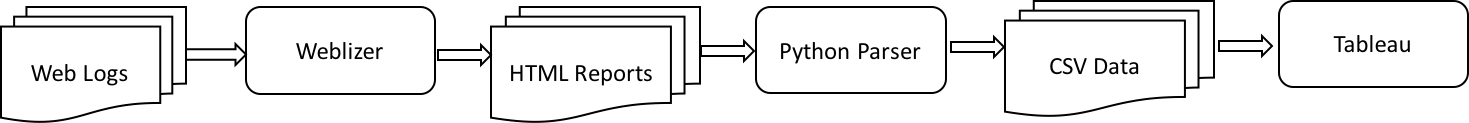
\includegraphics[width=\linewidth]{img/datapipeline.png}}
\caption{Data Pipeline.}
\label{fig:datapipeline}
\end{figure}


\subsection{Source Data} \label{sourcedata}
\begin{figure}
\centering
\fbox{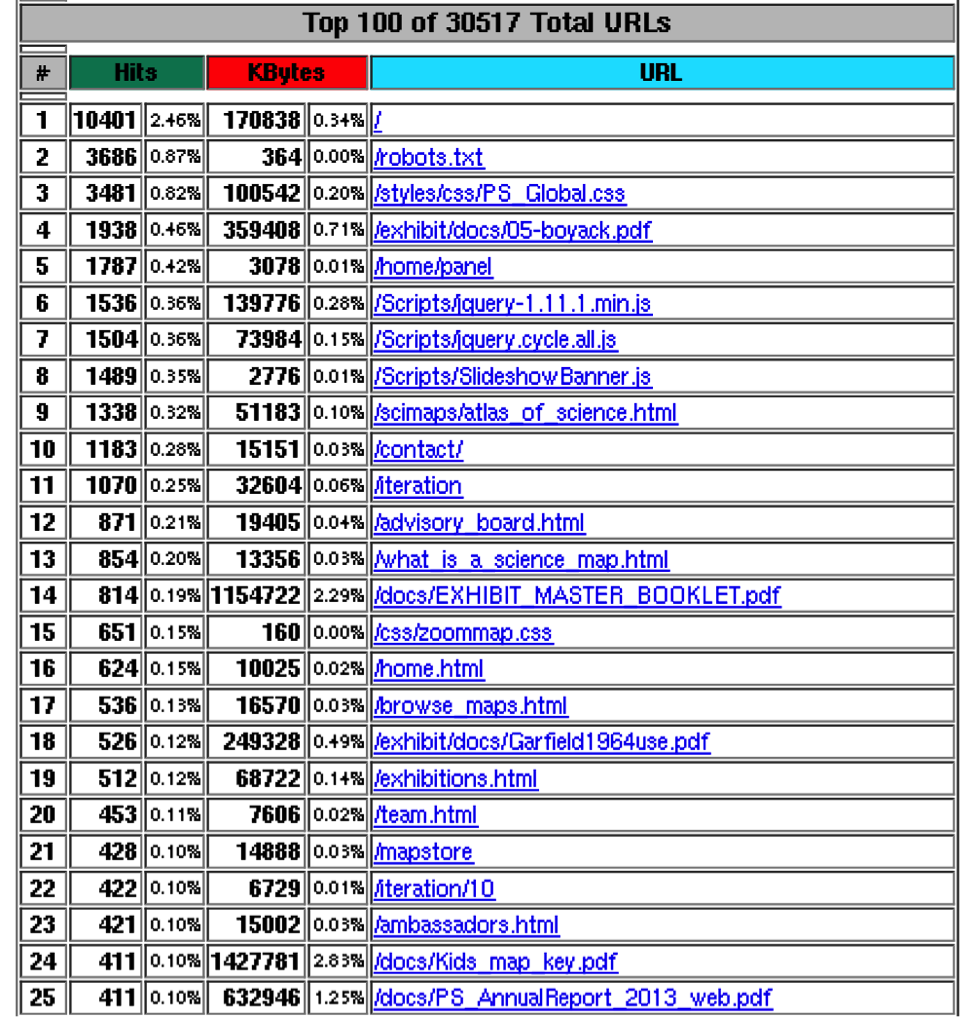
\includegraphics[width=\linewidth]{img/samplewebanalyzerreport.png}}
\caption{Sample Webanalyzer Report.}
\label{fig:samplewebanalyzer}
\end{figure}

As explained in section \ref{techsol}, the Webanalyzer reports in HTML format
are used as source data. These reports are available for last 10 years on
monthly basis. Each report has following sub-sections:
Monthly statistics, Daily statistics, Hourly statistics
, Top 100 URLs, Top 10 entry pages, Top 10 exit pages, Top 30 referring Sites, Top 20 search strings, Top 15 user agents, Top 10 countries

 Each section in webanalyzer report has HTML table. Figure
 \ref{fig:samplewebanalyzer} explains sample table from webanalyzer HTML
 report.


\subsection{Data Parser} \label{dataparser}
As explained in section \ref{techsol}, each Webanayzer HTML reports is
converted into CSV format. We implemented Data Parser Python script which
scrapes the
Webanalyzer HTML report and converts it into CSV structure. The data parser
uses Python module called BeautifulSoup to parse the HTML. It then iterates
over all 'A' tags to find the section header within HTML report. Finally it
iterates over the HTML table elements consisting TR and TD tags to extract
the data and writes it in CSV file.
 The data parser code is available at \cite{dataparser} repository. The
 figure \ref{fig:daystats} shows sample records from the DAYSTATS.csv which
 is one of the output CSV created by the data parser.

 \begin{figure}
\centering
\fbox{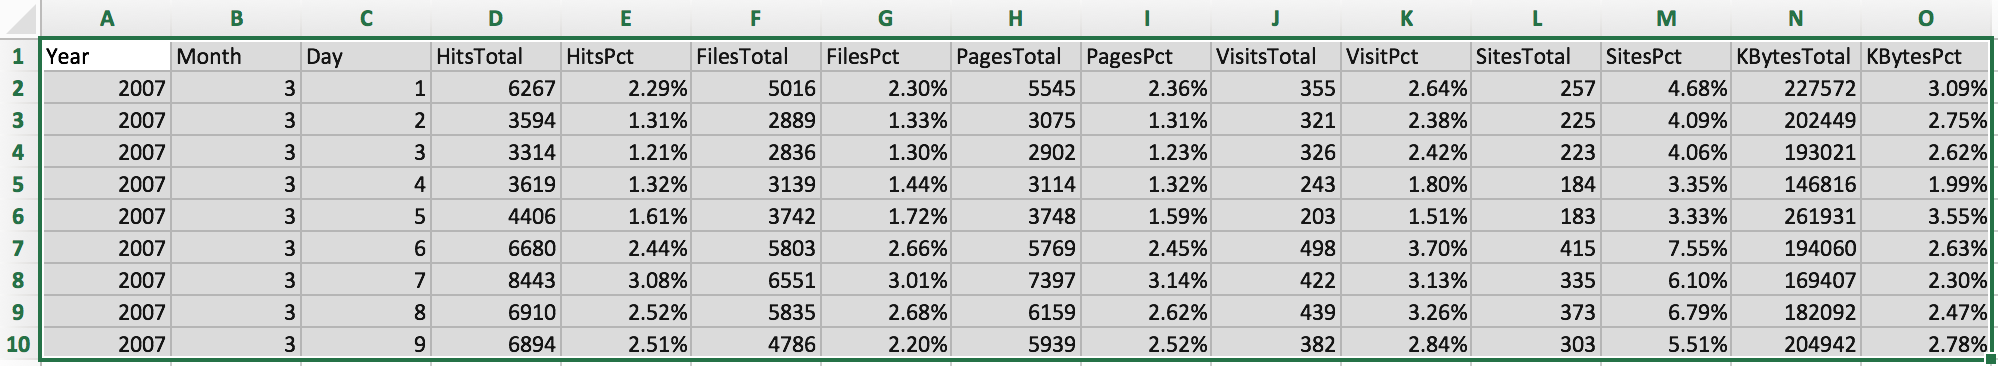
\includegraphics[width=\linewidth]{img/dailystats.png}}
\caption{Daily Statistics Sample Records.}
\label{fig:daystats}
\end{figure}





\section{Visualizations} \label{viz}
In this section, we explain various visualizations we created to satisfy the
project requirements. Section \ref{viz_dashboard} provides one page
interactive view of overall statistics whereas the subsequent visualizations
support detailed analysis of individual statistics.


\section{Key Insights} \label{keyinsights}

TODO: Leonard


\section{Conclusions}
"Lorem ipsum dolor sit amet, consectetur adipiscing elit, sed do eiusmod tempor incididunt ut labore et dolore magna aliqua. Ut enim ad minim veniam, quis nostrud exercitation ullamco laboris nisi ut aliquip ex ea commodo consequat. Duis aute irure dolor in reprehenderit in voluptate velit esse cillum dolore eu fugiat nulla pariatur. Excepteur sint occaecat cupidatat non proident, sunt in culpa qui officia deserunt mollit anim id est laborum."


%\end{document}  % This is where a 'short' article might terminate



\appendix
%Appendix A
%\section{Work Distribution}


\section{Acknowledgements}
 The authors thank Prof. Katy Börner for her technical guidance. The
 authors would also like to thank TAs of Information Visualization class for their valued
 support.


\bibliographystyle{ACM-Reference-Format}
\bibliography{main} 

\end{document}
